\documentclass[twoside]{book}

% Packages required by doxygen
\usepackage{calc}
\usepackage{doxygen}
\usepackage{graphicx}
\usepackage[utf8]{inputenc}
\usepackage{makeidx}
\usepackage{multicol}
\usepackage{multirow}
\usepackage{textcomp}
\usepackage[table]{xcolor}

% Font selection
\usepackage[T1]{fontenc}
\usepackage{mathptmx}
\usepackage[scaled=.90]{helvet}
\usepackage{courier}
\usepackage{amssymb}
\usepackage{sectsty}
\renewcommand{\familydefault}{\sfdefault}
\allsectionsfont{%
  \fontseries{bc}\selectfont%
  \color{darkgray}%
}
\renewcommand{\DoxyLabelFont}{%
  \fontseries{bc}\selectfont%
  \color{darkgray}%
}

% Page & text layout
\usepackage{geometry}
\geometry{%
  a4paper,%
  top=2.5cm,%
  bottom=2.5cm,%
  left=2.5cm,%
  right=2.5cm%
}
\tolerance=750
\hfuzz=15pt
\hbadness=750
\setlength{\emergencystretch}{15pt}
\setlength{\parindent}{0cm}
\setlength{\parskip}{0.2cm}
\makeatletter
\renewcommand{\paragraph}{%
  \@startsection{paragraph}{4}{0ex}{-1.0ex}{1.0ex}{%
    \normalfont\normalsize\bfseries\SS@parafont%
  }%
}
\renewcommand{\subparagraph}{%
  \@startsection{subparagraph}{5}{0ex}{-1.0ex}{1.0ex}{%
    \normalfont\normalsize\bfseries\SS@subparafont%
  }%
}
\makeatother

% Headers & footers
\usepackage{fancyhdr}
\pagestyle{fancyplain}
\fancyhead[LE]{\fancyplain{}{\bfseries\thepage}}
\fancyhead[CE]{\fancyplain{}{}}
\fancyhead[RE]{\fancyplain{}{\bfseries\leftmark}}
\fancyhead[LO]{\fancyplain{}{\bfseries\rightmark}}
\fancyhead[CO]{\fancyplain{}{}}
\fancyhead[RO]{\fancyplain{}{\bfseries\thepage}}
\fancyfoot[LE]{\fancyplain{}{}}
\fancyfoot[CE]{\fancyplain{}{}}
\fancyfoot[RE]{\fancyplain{}{\bfseries\scriptsize Generated on Thu Dec 13 2018 22\-:58\-:43 for Auto\-Di\-F\-K by Doxygen }}
\fancyfoot[LO]{\fancyplain{}{\bfseries\scriptsize Generated on Thu Dec 13 2018 22\-:58\-:43 for Auto\-Di\-F\-K by Doxygen }}
\fancyfoot[CO]{\fancyplain{}{}}
\fancyfoot[RO]{\fancyplain{}{}}
\renewcommand{\footrulewidth}{0.4pt}
\renewcommand{\chaptermark}[1]{%
  \markboth{#1}{}%
}
\renewcommand{\sectionmark}[1]{%
  \markright{\thesection\ #1}%
}

% Indices & bibliography
\usepackage{natbib}
\usepackage[titles]{tocloft}
\setcounter{tocdepth}{3}
\setcounter{secnumdepth}{5}
\makeindex

% Hyperlinks (required, but should be loaded last)
\usepackage{ifpdf}
\ifpdf
  \usepackage[pdftex,pagebackref=true]{hyperref}
\else
  \usepackage[ps2pdf,pagebackref=true]{hyperref}
\fi
\hypersetup{%
  colorlinks=true,%
  linkcolor=blue,%
  citecolor=blue,%
  unicode%
}

% Custom commands
\newcommand{\clearemptydoublepage}{%
  \newpage{\pagestyle{empty}\cleardoublepage}%
}


%===== C O N T E N T S =====

\begin{document}

% Titlepage & ToC
\hypersetup{pageanchor=false}
\pagenumbering{roman}
\begin{titlepage}
\vspace*{7cm}
\begin{center}%
{\Large Auto\-Di\-F\-K }\\
\vspace*{1cm}
{\large Generated by Doxygen 1.8.6}\\
\vspace*{0.5cm}
{\small Thu Dec 13 2018 22:58:43}\\
\end{center}
\end{titlepage}
\clearemptydoublepage
\tableofcontents
\clearemptydoublepage
\pagenumbering{arabic}
\hypersetup{pageanchor=true}

%--- Begin generated contents ---
\chapter{Hierarchical Index}
\section{Class Hierarchy}
This inheritance list is sorted roughly, but not completely, alphabetically\-:\begin{DoxyCompactList}
\item \contentsline{section}{autodifk\-:\-:forward\-:\-:Dual\-Scalar}{\pageref{structautodifk_1_1forward_1_1_dual_scalar}}{}
\item \contentsline{section}{autodifk\-:\-:forward\-:\-:Forward\-Autodiff$<$ F, N\-\_\-\-I\-N\-P\-U\-T\-S, N\-\_\-\-O\-U\-T\-P\-U\-T\-S $>$}{\pageref{classautodifk_1_1forward_1_1_forward_autodiff}}{}
\item \contentsline{section}{autodifk\-:\-:Numerical\-Diff$<$ F, N\-\_\-\-I\-N\-P\-U\-T\-S, N\-\_\-\-O\-U\-T\-P\-U\-T\-S $>$}{\pageref{classautodifk_1_1_numerical_diff}}{}
\item \contentsline{section}{autodifk\-:\-:reverse\-:\-:Scalar\-Expression}{\pageref{classautodifk_1_1reverse_1_1_scalar_expression}}{}
\begin{DoxyCompactList}
\item \contentsline{section}{autodifk\-:\-:reverse\-:\-:Constant\-Scalar\-Expression}{\pageref{classautodifk_1_1reverse_1_1_constant_scalar_expression}}{}
\item \contentsline{section}{autodifk\-:\-:reverse\-:\-:Product}{\pageref{classautodifk_1_1reverse_1_1_product}}{}
\item \contentsline{section}{autodifk\-:\-:reverse\-:\-:Sum}{\pageref{classautodifk_1_1reverse_1_1_sum}}{}
\item \contentsline{section}{autodifk\-:\-:reverse\-:\-:Unary\-Scalar\-Expression}{\pageref{classautodifk_1_1reverse_1_1_unary_scalar_expression}}{}
\begin{DoxyCompactList}
\item \contentsline{section}{autodifk\-:\-:reverse\-:\-:Abs}{\pageref{classautodifk_1_1reverse_1_1_abs}}{}
\item \contentsline{section}{autodifk\-:\-:reverse\-:\-:Cos}{\pageref{classautodifk_1_1reverse_1_1_cos}}{}
\item \contentsline{section}{autodifk\-:\-:reverse\-:\-:Exp}{\pageref{classautodifk_1_1reverse_1_1_exp}}{}
\item \contentsline{section}{autodifk\-:\-:reverse\-:\-:Log}{\pageref{classautodifk_1_1reverse_1_1_log}}{}
\item \contentsline{section}{autodifk\-:\-:reverse\-:\-:Re\-L\-U}{\pageref{classautodifk_1_1reverse_1_1_re_l_u}}{}
\item \contentsline{section}{autodifk\-:\-:reverse\-:\-:Sin}{\pageref{classautodifk_1_1reverse_1_1_sin}}{}
\item \contentsline{section}{autodifk\-:\-:reverse\-:\-:Tan}{\pageref{classautodifk_1_1reverse_1_1_tan}}{}
\end{DoxyCompactList}
\end{DoxyCompactList}
\end{DoxyCompactList}

\chapter{Class Index}
\section{Class List}
Here are the classes, structs, unions and interfaces with brief descriptions\-:\begin{DoxyCompactList}
\item\contentsline{section}{\hyperlink{classautodifk_1_1reverse_1_1_abs}{autodifk\-::reverse\-::\-Abs} }{\pageref{classautodifk_1_1reverse_1_1_abs}}{}
\item\contentsline{section}{\hyperlink{classautodifk_1_1reverse_1_1_constant_scalar_expression}{autodifk\-::reverse\-::\-Constant\-Scalar\-Expression} }{\pageref{classautodifk_1_1reverse_1_1_constant_scalar_expression}}{}
\item\contentsline{section}{\hyperlink{classautodifk_1_1reverse_1_1_cos}{autodifk\-::reverse\-::\-Cos} }{\pageref{classautodifk_1_1reverse_1_1_cos}}{}
\item\contentsline{section}{\hyperlink{structautodifk_1_1forward_1_1_dual_scalar}{autodifk\-::forward\-::\-Dual\-Scalar} }{\pageref{structautodifk_1_1forward_1_1_dual_scalar}}{}
\item\contentsline{section}{\hyperlink{classautodifk_1_1reverse_1_1_exp}{autodifk\-::reverse\-::\-Exp} }{\pageref{classautodifk_1_1reverse_1_1_exp}}{}
\item\contentsline{section}{\hyperlink{classautodifk_1_1forward_1_1_forward_autodiff}{autodifk\-::forward\-::\-Forward\-Autodiff$<$ F, N\-\_\-\-I\-N\-P\-U\-T\-S, N\-\_\-\-O\-U\-T\-P\-U\-T\-S $>$} }{\pageref{classautodifk_1_1forward_1_1_forward_autodiff}}{}
\item\contentsline{section}{\hyperlink{classautodifk_1_1reverse_1_1_log}{autodifk\-::reverse\-::\-Log} }{\pageref{classautodifk_1_1reverse_1_1_log}}{}
\item\contentsline{section}{\hyperlink{classautodifk_1_1_numerical_diff}{autodifk\-::\-Numerical\-Diff$<$ F, N\-\_\-\-I\-N\-P\-U\-T\-S, N\-\_\-\-O\-U\-T\-P\-U\-T\-S $>$} }{\pageref{classautodifk_1_1_numerical_diff}}{}
\item\contentsline{section}{\hyperlink{classautodifk_1_1reverse_1_1_product}{autodifk\-::reverse\-::\-Product} }{\pageref{classautodifk_1_1reverse_1_1_product}}{}
\item\contentsline{section}{\hyperlink{classautodifk_1_1reverse_1_1_re_l_u}{autodifk\-::reverse\-::\-Re\-L\-U} }{\pageref{classautodifk_1_1reverse_1_1_re_l_u}}{}
\item\contentsline{section}{\hyperlink{classautodifk_1_1reverse_1_1_scalar_expression}{autodifk\-::reverse\-::\-Scalar\-Expression} }{\pageref{classautodifk_1_1reverse_1_1_scalar_expression}}{}
\item\contentsline{section}{\hyperlink{classautodifk_1_1reverse_1_1_sin}{autodifk\-::reverse\-::\-Sin} }{\pageref{classautodifk_1_1reverse_1_1_sin}}{}
\item\contentsline{section}{\hyperlink{classautodifk_1_1reverse_1_1_sum}{autodifk\-::reverse\-::\-Sum} }{\pageref{classautodifk_1_1reverse_1_1_sum}}{}
\item\contentsline{section}{\hyperlink{classautodifk_1_1reverse_1_1_tan}{autodifk\-::reverse\-::\-Tan} }{\pageref{classautodifk_1_1reverse_1_1_tan}}{}
\item\contentsline{section}{\hyperlink{classautodifk_1_1reverse_1_1_unary_scalar_expression}{autodifk\-::reverse\-::\-Unary\-Scalar\-Expression} }{\pageref{classautodifk_1_1reverse_1_1_unary_scalar_expression}}{}
\end{DoxyCompactList}

\chapter{Class Documentation}
\hypertarget{classautodifk_1_1reverse_1_1_abs}{\section{autodifk\-:\-:reverse\-:\-:Abs Class Reference}
\label{classautodifk_1_1reverse_1_1_abs}\index{autodifk\-::reverse\-::\-Abs@{autodifk\-::reverse\-::\-Abs}}
}
Inheritance diagram for autodifk\-:\-:reverse\-:\-:Abs\-:\begin{figure}[H]
\begin{center}
\leavevmode
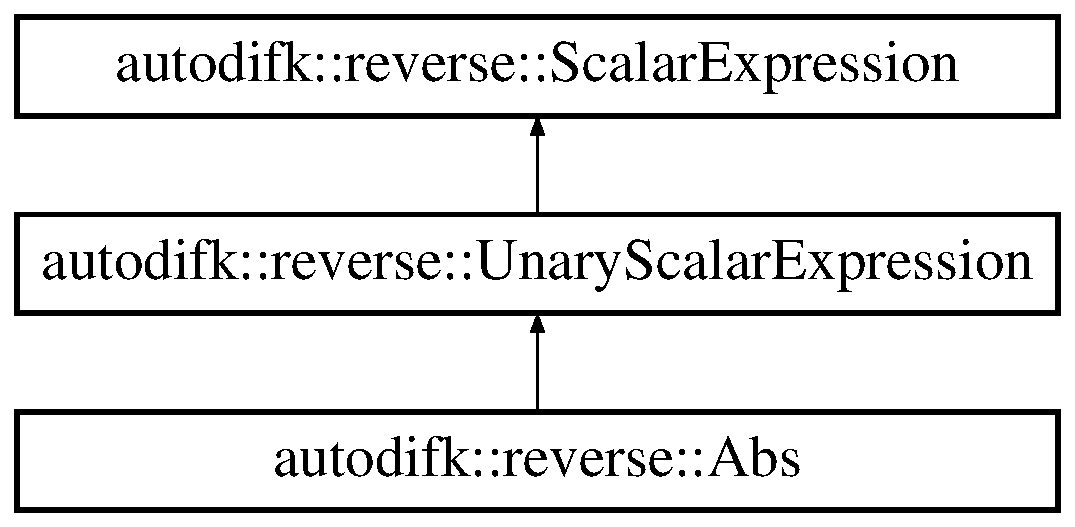
\includegraphics[height=3.000000cm]{classautodifk_1_1reverse_1_1_abs}
\end{center}
\end{figure}
\subsection*{Public Types}
\begin{DoxyCompactItemize}
\item 
\hypertarget{classautodifk_1_1reverse_1_1_abs_a1fe7cfa1fda1b9a91f4de60ed384c5db}{typedef std\-::shared\-\_\-ptr$<$ \hyperlink{classautodifk_1_1reverse_1_1_abs}{Abs} $>$ {\bfseries Ptr}}\label{classautodifk_1_1reverse_1_1_abs_a1fe7cfa1fda1b9a91f4de60ed384c5db}

\item 
\hypertarget{classautodifk_1_1reverse_1_1_abs_a670da446cde5341249ef5427b8583a7c}{typedef std\-::shared\-\_\-ptr$<$ const \\*
\hyperlink{classautodifk_1_1reverse_1_1_abs}{Abs} $>$ {\bfseries Const\-Ptr}}\label{classautodifk_1_1reverse_1_1_abs_a670da446cde5341249ef5427b8583a7c}

\end{DoxyCompactItemize}
\subsection*{Static Public Member Functions}
\begin{DoxyCompactItemize}
\item 
\hypertarget{classautodifk_1_1reverse_1_1_abs_a8b17fb02413baf6e0d66ebf07cd53897}{static Ptr {\bfseries Create} (const std\-::vector$<$ Scalar\-Expression\-::\-Ptr $>$ \&subexpressions)}\label{classautodifk_1_1reverse_1_1_abs_a8b17fb02413baf6e0d66ebf07cd53897}

\item 
\hypertarget{classautodifk_1_1reverse_1_1_abs_a9b2cb0ed31387b12623d9a0dd1cefcd1}{static Ptr {\bfseries Create} (const std\-::initializer\-\_\-list$<$ Scalar\-Expression\-::\-Ptr $>$ \&subexpressions)}\label{classautodifk_1_1reverse_1_1_abs_a9b2cb0ed31387b12623d9a0dd1cefcd1}

\end{DoxyCompactItemize}
\subsection*{Additional Inherited Members}


\subsection{Detailed Description}


Definition at line 195 of file utils.\-h.



The documentation for this class was generated from the following files\-:\begin{DoxyCompactItemize}
\item 
/home/travis/build/dfridovi/autodifk/include/reverse/utils.\-h\item 
/home/travis/build/dfridovi/autodifk/src/reverse/utils.\-cpp\end{DoxyCompactItemize}

\hypertarget{classautodifk_1_1reverse_1_1_constant_scalar_expression}{\section{autodifk\-:\-:reverse\-:\-:Constant\-Scalar\-Expression Class Reference}
\label{classautodifk_1_1reverse_1_1_constant_scalar_expression}\index{autodifk\-::reverse\-::\-Constant\-Scalar\-Expression@{autodifk\-::reverse\-::\-Constant\-Scalar\-Expression}}
}
Inheritance diagram for autodifk\-:\-:reverse\-:\-:Constant\-Scalar\-Expression\-:\begin{figure}[H]
\begin{center}
\leavevmode
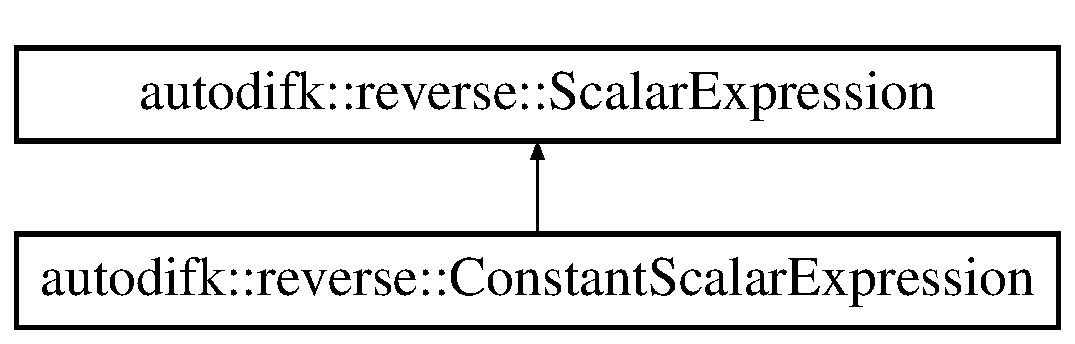
\includegraphics[height=2.000000cm]{classautodifk_1_1reverse_1_1_constant_scalar_expression}
\end{center}
\end{figure}
\subsection*{Public Types}
\begin{DoxyCompactItemize}
\item 
\hypertarget{classautodifk_1_1reverse_1_1_constant_scalar_expression_abfe0e0ee401cbef9e89ba750f78de53e}{typedef std\-::shared\-\_\-ptr\\*
$<$ \hyperlink{classautodifk_1_1reverse_1_1_constant_scalar_expression}{Constant\-Scalar\-Expression} $>$ {\bfseries Ptr}}\label{classautodifk_1_1reverse_1_1_constant_scalar_expression_abfe0e0ee401cbef9e89ba750f78de53e}

\item 
\hypertarget{classautodifk_1_1reverse_1_1_constant_scalar_expression_aa7369d7143a4b60b070c1fccfd96935a}{typedef std\-::shared\-\_\-ptr$<$ const \\*
\hyperlink{classautodifk_1_1reverse_1_1_constant_scalar_expression}{Constant\-Scalar\-Expression} $>$ {\bfseries Const\-Ptr}}\label{classautodifk_1_1reverse_1_1_constant_scalar_expression_aa7369d7143a4b60b070c1fccfd96935a}

\end{DoxyCompactItemize}
\subsection*{Static Public Member Functions}
\begin{DoxyCompactItemize}
\item 
\hypertarget{classautodifk_1_1reverse_1_1_constant_scalar_expression_a0408fecd73c15d83ef9bd23dd0af7c09}{static Ptr {\bfseries Create} ()}\label{classautodifk_1_1reverse_1_1_constant_scalar_expression_a0408fecd73c15d83ef9bd23dd0af7c09}

\item 
\hypertarget{classautodifk_1_1reverse_1_1_constant_scalar_expression_a58c272a8761a2939d387616ef090a45a}{static Ptr {\bfseries Create} (double v)}\label{classautodifk_1_1reverse_1_1_constant_scalar_expression_a58c272a8761a2939d387616ef090a45a}

\end{DoxyCompactItemize}
\subsection*{Additional Inherited Members}


\subsection{Detailed Description}


Definition at line 155 of file scalar\-\_\-expression.\-h.



The documentation for this class was generated from the following file\-:\begin{DoxyCompactItemize}
\item 
/home/travis/build/dfridovi/autodifk/include/reverse/scalar\-\_\-expression.\-h\end{DoxyCompactItemize}

\hypertarget{classautodifk_1_1reverse_1_1_cos}{\section{autodifk\-:\-:reverse\-:\-:Cos Class Reference}
\label{classautodifk_1_1reverse_1_1_cos}\index{autodifk\-::reverse\-::\-Cos@{autodifk\-::reverse\-::\-Cos}}
}
Inheritance diagram for autodifk\-:\-:reverse\-:\-:Cos\-:\begin{figure}[H]
\begin{center}
\leavevmode
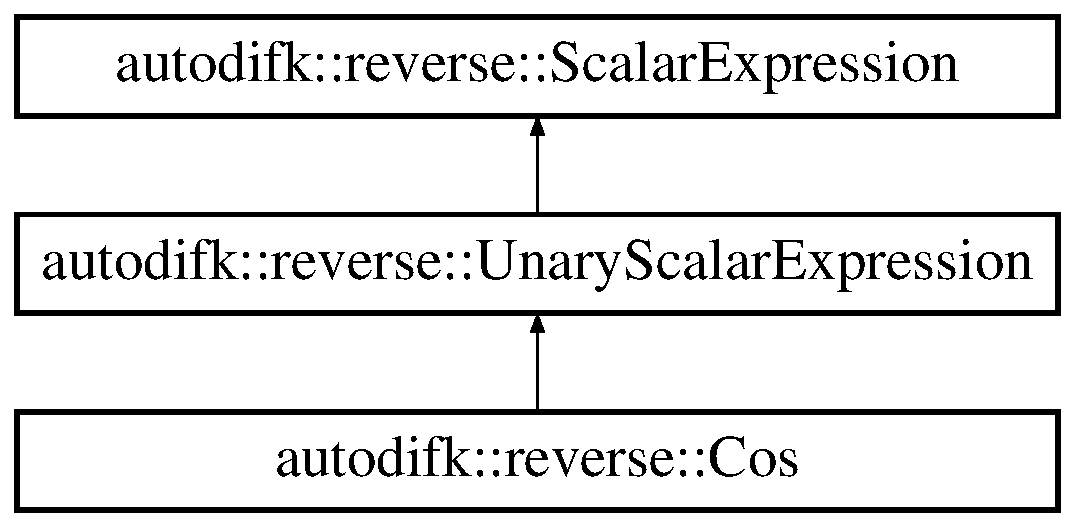
\includegraphics[height=3.000000cm]{classautodifk_1_1reverse_1_1_cos}
\end{center}
\end{figure}
\subsection*{Public Types}
\begin{DoxyCompactItemize}
\item 
\hypertarget{classautodifk_1_1reverse_1_1_cos_a51a1b4db9026e1f4b6587cf903d58a55}{typedef std\-::shared\-\_\-ptr$<$ \hyperlink{classautodifk_1_1reverse_1_1_cos}{Cos} $>$ {\bfseries Ptr}}\label{classautodifk_1_1reverse_1_1_cos_a51a1b4db9026e1f4b6587cf903d58a55}

\item 
\hypertarget{classautodifk_1_1reverse_1_1_cos_aba4bb9a43267a07f3abd8d4e83968d5e}{typedef std\-::shared\-\_\-ptr$<$ const \\*
\hyperlink{classautodifk_1_1reverse_1_1_cos}{Cos} $>$ {\bfseries Const\-Ptr}}\label{classautodifk_1_1reverse_1_1_cos_aba4bb9a43267a07f3abd8d4e83968d5e}

\end{DoxyCompactItemize}
\subsection*{Static Public Member Functions}
\begin{DoxyCompactItemize}
\item 
\hypertarget{classautodifk_1_1reverse_1_1_cos_a7a6faa6d27028983a4f6242ac85a51b3}{static Ptr {\bfseries Create} (const std\-::vector$<$ Scalar\-Expression\-::\-Ptr $>$ \&subexpressions)}\label{classautodifk_1_1reverse_1_1_cos_a7a6faa6d27028983a4f6242ac85a51b3}

\item 
\hypertarget{classautodifk_1_1reverse_1_1_cos_af3e6e1d3a3e15f68c71ad7c02c862a32}{static Ptr {\bfseries Create} (const std\-::initializer\-\_\-list$<$ Scalar\-Expression\-::\-Ptr $>$ \&subexpressions)}\label{classautodifk_1_1reverse_1_1_cos_af3e6e1d3a3e15f68c71ad7c02c862a32}

\end{DoxyCompactItemize}
\subsection*{Additional Inherited Members}


\subsection{Detailed Description}


Definition at line 115 of file utils.\-h.



The documentation for this class was generated from the following files\-:\begin{DoxyCompactItemize}
\item 
/home/travis/build/dfridovi/autodifk/include/reverse/utils.\-h\item 
/home/travis/build/dfridovi/autodifk/src/reverse/utils.\-cpp\end{DoxyCompactItemize}

\hypertarget{structautodifk_1_1forward_1_1_dual_scalar}{\section{autodifk\-:\-:forward\-:\-:Dual\-Scalar Struct Reference}
\label{structautodifk_1_1forward_1_1_dual_scalar}\index{autodifk\-::forward\-::\-Dual\-Scalar@{autodifk\-::forward\-::\-Dual\-Scalar}}
}
\subsection*{Public Member Functions}
\begin{DoxyCompactItemize}
\item 
\hypertarget{structautodifk_1_1forward_1_1_dual_scalar_a644f21b9238e1492c87dbf2410aaa429}{{\bfseries Dual\-Scalar} (double v)}\label{structautodifk_1_1forward_1_1_dual_scalar_a644f21b9238e1492c87dbf2410aaa429}

\item 
\hypertarget{structautodifk_1_1forward_1_1_dual_scalar_aa18242f5946144ace77cbd911d0d3f9f}{{\bfseries Dual\-Scalar} (double v, double d)}\label{structautodifk_1_1forward_1_1_dual_scalar_aa18242f5946144ace77cbd911d0d3f9f}

\item 
\hypertarget{structautodifk_1_1forward_1_1_dual_scalar_aa5ecf8d86d75273eef402bbd27578304}{\hyperlink{structautodifk_1_1forward_1_1_dual_scalar}{Dual\-Scalar} {\bfseries operator-\/} () const }\label{structautodifk_1_1forward_1_1_dual_scalar_aa5ecf8d86d75273eef402bbd27578304}

\item 
\hypertarget{structautodifk_1_1forward_1_1_dual_scalar_ad81932a8fda687d7dc87741363f0ecba}{\hyperlink{structautodifk_1_1forward_1_1_dual_scalar}{Dual\-Scalar} \& {\bfseries operator+=} (const \hyperlink{structautodifk_1_1forward_1_1_dual_scalar}{Dual\-Scalar} \&rhs)}\label{structautodifk_1_1forward_1_1_dual_scalar_ad81932a8fda687d7dc87741363f0ecba}

\item 
\hypertarget{structautodifk_1_1forward_1_1_dual_scalar_a44f50035ebb486e8610d5da01b5900e6}{\hyperlink{structautodifk_1_1forward_1_1_dual_scalar}{Dual\-Scalar} \& {\bfseries operator-\/=} (const \hyperlink{structautodifk_1_1forward_1_1_dual_scalar}{Dual\-Scalar} \&rhs)}\label{structautodifk_1_1forward_1_1_dual_scalar_a44f50035ebb486e8610d5da01b5900e6}

\item 
\hypertarget{structautodifk_1_1forward_1_1_dual_scalar_ab58fd4d4e986d0dc8d6a5a433fa9a48e}{\hyperlink{structautodifk_1_1forward_1_1_dual_scalar}{Dual\-Scalar} \& {\bfseries operator$\ast$=} (const \hyperlink{structautodifk_1_1forward_1_1_dual_scalar}{Dual\-Scalar} \&rhs)}\label{structautodifk_1_1forward_1_1_dual_scalar_ab58fd4d4e986d0dc8d6a5a433fa9a48e}

\item 
\hypertarget{structautodifk_1_1forward_1_1_dual_scalar_a4460eee6e05601ff7b254d98ece3f9c6}{\hyperlink{structautodifk_1_1forward_1_1_dual_scalar}{Dual\-Scalar} \& {\bfseries operator/=} (const \hyperlink{structautodifk_1_1forward_1_1_dual_scalar}{Dual\-Scalar} \&rhs)}\label{structautodifk_1_1forward_1_1_dual_scalar_a4460eee6e05601ff7b254d98ece3f9c6}

\end{DoxyCompactItemize}
\subsection*{Public Attributes}
\begin{DoxyCompactItemize}
\item 
\hypertarget{structautodifk_1_1forward_1_1_dual_scalar_a7b05a23f4e01fd8b3ed1183539b44291}{double {\bfseries value}}\label{structautodifk_1_1forward_1_1_dual_scalar_a7b05a23f4e01fd8b3ed1183539b44291}

\item 
\hypertarget{structautodifk_1_1forward_1_1_dual_scalar_ae9baa4e80b012e4abd632c02a9e8bb01}{double {\bfseries derivative}}\label{structautodifk_1_1forward_1_1_dual_scalar_ae9baa4e80b012e4abd632c02a9e8bb01}

\end{DoxyCompactItemize}
\subsection*{Friends}
\begin{DoxyCompactItemize}
\item 
\hypertarget{structautodifk_1_1forward_1_1_dual_scalar_aab69c270c3a1a63162cb30c8024d0805}{\hyperlink{structautodifk_1_1forward_1_1_dual_scalar}{Dual\-Scalar} {\bfseries operator+} (\hyperlink{structautodifk_1_1forward_1_1_dual_scalar}{Dual\-Scalar} lhs, const \hyperlink{structautodifk_1_1forward_1_1_dual_scalar}{Dual\-Scalar} \&rhs)}\label{structautodifk_1_1forward_1_1_dual_scalar_aab69c270c3a1a63162cb30c8024d0805}

\item 
\hypertarget{structautodifk_1_1forward_1_1_dual_scalar_a1ca8db808079745f55941dbde1c8105a}{\hyperlink{structautodifk_1_1forward_1_1_dual_scalar}{Dual\-Scalar} {\bfseries operator-\/} (\hyperlink{structautodifk_1_1forward_1_1_dual_scalar}{Dual\-Scalar} lhs, const \hyperlink{structautodifk_1_1forward_1_1_dual_scalar}{Dual\-Scalar} \&rhs)}\label{structautodifk_1_1forward_1_1_dual_scalar_a1ca8db808079745f55941dbde1c8105a}

\item 
\hypertarget{structautodifk_1_1forward_1_1_dual_scalar_a14b2dac1e347eda91210a88b283eb716}{\hyperlink{structautodifk_1_1forward_1_1_dual_scalar}{Dual\-Scalar} {\bfseries operator$\ast$} (\hyperlink{structautodifk_1_1forward_1_1_dual_scalar}{Dual\-Scalar} lhs, const \hyperlink{structautodifk_1_1forward_1_1_dual_scalar}{Dual\-Scalar} \&rhs)}\label{structautodifk_1_1forward_1_1_dual_scalar_a14b2dac1e347eda91210a88b283eb716}

\item 
\hypertarget{structautodifk_1_1forward_1_1_dual_scalar_a52b88fd20816fe8748deca2d2c442fa1}{\hyperlink{structautodifk_1_1forward_1_1_dual_scalar}{Dual\-Scalar} {\bfseries operator/} (\hyperlink{structautodifk_1_1forward_1_1_dual_scalar}{Dual\-Scalar} lhs, const \hyperlink{structautodifk_1_1forward_1_1_dual_scalar}{Dual\-Scalar} \&rhs)}\label{structautodifk_1_1forward_1_1_dual_scalar_a52b88fd20816fe8748deca2d2c442fa1}

\item 
\hypertarget{structautodifk_1_1forward_1_1_dual_scalar_a22976b0f4675b7bc229ad55c2ed52291}{bool {\bfseries operator==} (const \hyperlink{structautodifk_1_1forward_1_1_dual_scalar}{Dual\-Scalar} \&lhs, const \hyperlink{structautodifk_1_1forward_1_1_dual_scalar}{Dual\-Scalar} \&rhs)}\label{structautodifk_1_1forward_1_1_dual_scalar_a22976b0f4675b7bc229ad55c2ed52291}

\item 
\hypertarget{structautodifk_1_1forward_1_1_dual_scalar_aaee9f7e5aae1478510ae5a600fbf731c}{bool {\bfseries operator!=} (const \hyperlink{structautodifk_1_1forward_1_1_dual_scalar}{Dual\-Scalar} \&lhs, const \hyperlink{structautodifk_1_1forward_1_1_dual_scalar}{Dual\-Scalar} \&rhs)}\label{structautodifk_1_1forward_1_1_dual_scalar_aaee9f7e5aae1478510ae5a600fbf731c}

\item 
\hypertarget{structautodifk_1_1forward_1_1_dual_scalar_a4d17a1fd2cfbf6e25e9a41faf628eb89}{bool {\bfseries operator$<$} (const \hyperlink{structautodifk_1_1forward_1_1_dual_scalar}{Dual\-Scalar} \&lhs, const \hyperlink{structautodifk_1_1forward_1_1_dual_scalar}{Dual\-Scalar} \&rhs)}\label{structautodifk_1_1forward_1_1_dual_scalar_a4d17a1fd2cfbf6e25e9a41faf628eb89}

\item 
\hypertarget{structautodifk_1_1forward_1_1_dual_scalar_aaf25c9a7e82161137ab26bb950ea2ef0}{bool {\bfseries operator$<$=} (const \hyperlink{structautodifk_1_1forward_1_1_dual_scalar}{Dual\-Scalar} \&lhs, const \hyperlink{structautodifk_1_1forward_1_1_dual_scalar}{Dual\-Scalar} \&rhs)}\label{structautodifk_1_1forward_1_1_dual_scalar_aaf25c9a7e82161137ab26bb950ea2ef0}

\item 
\hypertarget{structautodifk_1_1forward_1_1_dual_scalar_ae6a690f333d5990f1e951f7854116439}{bool {\bfseries operator$>$} (const \hyperlink{structautodifk_1_1forward_1_1_dual_scalar}{Dual\-Scalar} \&lhs, const \hyperlink{structautodifk_1_1forward_1_1_dual_scalar}{Dual\-Scalar} \&rhs)}\label{structautodifk_1_1forward_1_1_dual_scalar_ae6a690f333d5990f1e951f7854116439}

\item 
\hypertarget{structautodifk_1_1forward_1_1_dual_scalar_accce569fb424fe941de94ababf797f1f}{bool {\bfseries operator$>$=} (const \hyperlink{structautodifk_1_1forward_1_1_dual_scalar}{Dual\-Scalar} \&lhs, const \hyperlink{structautodifk_1_1forward_1_1_dual_scalar}{Dual\-Scalar} \&rhs)}\label{structautodifk_1_1forward_1_1_dual_scalar_accce569fb424fe941de94ababf797f1f}

\item 
\hypertarget{structautodifk_1_1forward_1_1_dual_scalar_a80e063d53875f05090676f54f6d1a497}{std\-::ostream \& {\bfseries operator$<$$<$} (std\-::ostream \&out, const \hyperlink{structautodifk_1_1forward_1_1_dual_scalar}{Dual\-Scalar} \&rhs)}\label{structautodifk_1_1forward_1_1_dual_scalar_a80e063d53875f05090676f54f6d1a497}

\end{DoxyCompactItemize}


\subsection{Detailed Description}


Definition at line 55 of file dual\-\_\-scalar.\-h.



The documentation for this struct was generated from the following file\-:\begin{DoxyCompactItemize}
\item 
/home/travis/build/dfridovi/autodifk/include/forward/dual\-\_\-scalar.\-h\end{DoxyCompactItemize}

\hypertarget{classautodifk_1_1reverse_1_1_exp}{\section{autodifk\-:\-:reverse\-:\-:Exp Class Reference}
\label{classautodifk_1_1reverse_1_1_exp}\index{autodifk\-::reverse\-::\-Exp@{autodifk\-::reverse\-::\-Exp}}
}
Inheritance diagram for autodifk\-:\-:reverse\-:\-:Exp\-:\begin{figure}[H]
\begin{center}
\leavevmode
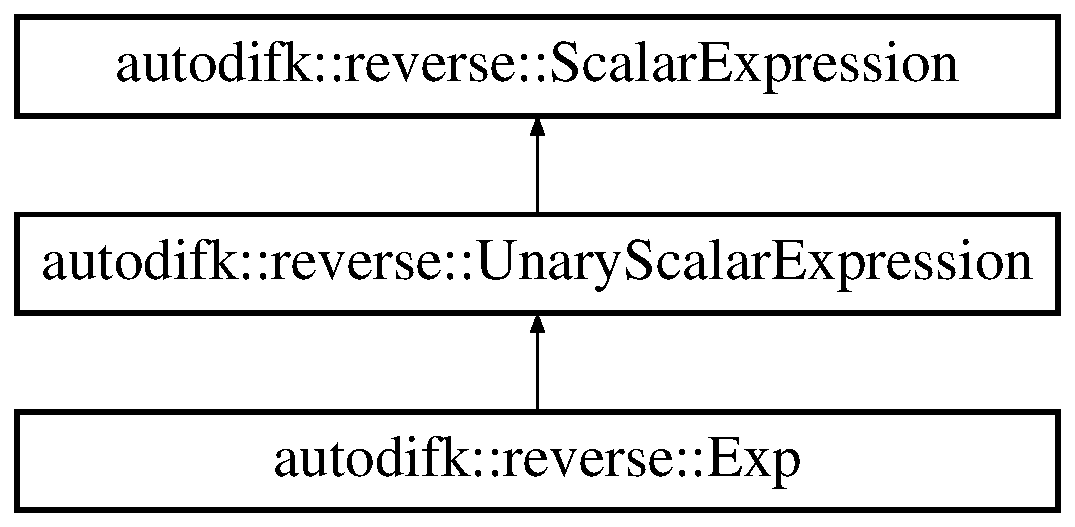
\includegraphics[height=3.000000cm]{classautodifk_1_1reverse_1_1_exp}
\end{center}
\end{figure}
\subsection*{Public Types}
\begin{DoxyCompactItemize}
\item 
\hypertarget{classautodifk_1_1reverse_1_1_exp_af6d692f52fd7e5ee8d7f1327823a3c1e}{typedef std\-::shared\-\_\-ptr$<$ \hyperlink{classautodifk_1_1reverse_1_1_exp}{Exp} $>$ {\bfseries Ptr}}\label{classautodifk_1_1reverse_1_1_exp_af6d692f52fd7e5ee8d7f1327823a3c1e}

\item 
\hypertarget{classautodifk_1_1reverse_1_1_exp_a78c046db213cc7a3ae0096a9de90a404}{typedef std\-::shared\-\_\-ptr$<$ const \\*
\hyperlink{classautodifk_1_1reverse_1_1_exp}{Exp} $>$ {\bfseries Const\-Ptr}}\label{classautodifk_1_1reverse_1_1_exp_a78c046db213cc7a3ae0096a9de90a404}

\end{DoxyCompactItemize}
\subsection*{Static Public Member Functions}
\begin{DoxyCompactItemize}
\item 
\hypertarget{classautodifk_1_1reverse_1_1_exp_af5c2b6af4679ec28449e6848a5749475}{static Ptr {\bfseries Create} (const std\-::vector$<$ Scalar\-Expression\-::\-Ptr $>$ \&subexpressions)}\label{classautodifk_1_1reverse_1_1_exp_af5c2b6af4679ec28449e6848a5749475}

\item 
\hypertarget{classautodifk_1_1reverse_1_1_exp_afb7c484df35a50d20c8533f7eafccbb2}{static Ptr {\bfseries Create} (const std\-::initializer\-\_\-list$<$ Scalar\-Expression\-::\-Ptr $>$ \&subexpressions)}\label{classautodifk_1_1reverse_1_1_exp_afb7c484df35a50d20c8533f7eafccbb2}

\end{DoxyCompactItemize}
\subsection*{Additional Inherited Members}


\subsection{Detailed Description}


Definition at line 155 of file utils.\-h.



The documentation for this class was generated from the following files\-:\begin{DoxyCompactItemize}
\item 
/home/travis/build/dfridovi/autodifk/include/reverse/utils.\-h\item 
/home/travis/build/dfridovi/autodifk/src/reverse/utils.\-cpp\end{DoxyCompactItemize}

\hypertarget{classautodifk_1_1forward_1_1_forward_autodiff}{\section{autodifk\-:\-:forward\-:\-:Forward\-Autodiff$<$ F, N\-\_\-\-I\-N\-P\-U\-T\-S, N\-\_\-\-O\-U\-T\-P\-U\-T\-S $>$ Class Template Reference}
\label{classautodifk_1_1forward_1_1_forward_autodiff}\index{autodifk\-::forward\-::\-Forward\-Autodiff$<$ F, N\-\_\-\-I\-N\-P\-U\-T\-S, N\-\_\-\-O\-U\-T\-P\-U\-T\-S $>$@{autodifk\-::forward\-::\-Forward\-Autodiff$<$ F, N\-\_\-\-I\-N\-P\-U\-T\-S, N\-\_\-\-O\-U\-T\-P\-U\-T\-S $>$}}
}
\subsection*{Public Member Functions}
\begin{DoxyCompactItemize}
\item 
\hypertarget{classautodifk_1_1forward_1_1_forward_autodiff_a9aacd8358aff72dd81fae26b027dbb74}{{\bfseries Forward\-Autodiff} (const F \&functor)}\label{classautodifk_1_1forward_1_1_forward_autodiff_a9aacd8358aff72dd81fae26b027dbb74}

\item 
\hypertarget{classautodifk_1_1forward_1_1_forward_autodiff_a5c75bf31f586588cee8d02a130f25104}{Eigen\-::\-Matrix$<$ double, \\*
N\-\_\-\-O\-U\-T\-P\-U\-T\-S, 1 $>$ {\bfseries Evaluate} (const Eigen\-::\-Matrix$<$ double, N\-\_\-\-I\-N\-P\-U\-T\-S, 1 $>$ \&x, Eigen\-::\-Matrix$<$ double, N\-\_\-\-O\-U\-T\-P\-U\-T\-S, N\-\_\-\-I\-N\-P\-U\-T\-S $>$ $\ast$jacobian)}\label{classautodifk_1_1forward_1_1_forward_autodiff_a5c75bf31f586588cee8d02a130f25104}

\end{DoxyCompactItemize}


\subsection{Detailed Description}
\subsubsection*{template$<$typename F, size\-\_\-t N\-\_\-\-I\-N\-P\-U\-T\-S, size\-\_\-t N\-\_\-\-O\-U\-T\-P\-U\-T\-S$>$class autodifk\-::forward\-::\-Forward\-Autodiff$<$ F, N\-\_\-\-I\-N\-P\-U\-T\-S, N\-\_\-\-O\-U\-T\-P\-U\-T\-S $>$}



Definition at line 58 of file forward\-\_\-autodiff.\-h.



The documentation for this class was generated from the following file\-:\begin{DoxyCompactItemize}
\item 
/home/travis/build/dfridovi/autodifk/include/forward/forward\-\_\-autodiff.\-h\end{DoxyCompactItemize}

\hypertarget{classautodifk_1_1reverse_1_1_log}{\section{autodifk\-:\-:reverse\-:\-:Log Class Reference}
\label{classautodifk_1_1reverse_1_1_log}\index{autodifk\-::reverse\-::\-Log@{autodifk\-::reverse\-::\-Log}}
}
Inheritance diagram for autodifk\-:\-:reverse\-:\-:Log\-:\begin{figure}[H]
\begin{center}
\leavevmode
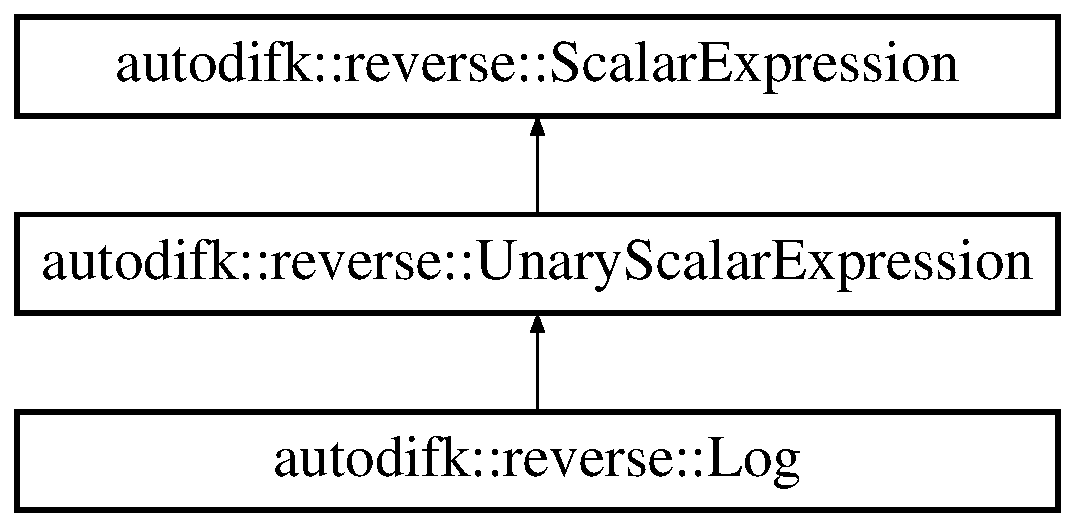
\includegraphics[height=3.000000cm]{classautodifk_1_1reverse_1_1_log}
\end{center}
\end{figure}
\subsection*{Public Types}
\begin{DoxyCompactItemize}
\item 
\hypertarget{classautodifk_1_1reverse_1_1_log_a9c1953ae1f3d91f14385aaa62cbe07c7}{typedef std\-::shared\-\_\-ptr$<$ \hyperlink{classautodifk_1_1reverse_1_1_log}{Log} $>$ {\bfseries Ptr}}\label{classautodifk_1_1reverse_1_1_log_a9c1953ae1f3d91f14385aaa62cbe07c7}

\item 
\hypertarget{classautodifk_1_1reverse_1_1_log_a7b424471b065614d4627584a50437a7b}{typedef std\-::shared\-\_\-ptr$<$ const \\*
\hyperlink{classautodifk_1_1reverse_1_1_log}{Log} $>$ {\bfseries Const\-Ptr}}\label{classautodifk_1_1reverse_1_1_log_a7b424471b065614d4627584a50437a7b}

\end{DoxyCompactItemize}
\subsection*{Static Public Member Functions}
\begin{DoxyCompactItemize}
\item 
\hypertarget{classautodifk_1_1reverse_1_1_log_af68dc69020ab0859dc9d87fe22ff52f0}{static Ptr {\bfseries Create} (const std\-::vector$<$ Scalar\-Expression\-::\-Ptr $>$ \&subexpressions)}\label{classautodifk_1_1reverse_1_1_log_af68dc69020ab0859dc9d87fe22ff52f0}

\item 
\hypertarget{classautodifk_1_1reverse_1_1_log_ad0ceeaf7e6152a55d0202419fb571802}{static Ptr {\bfseries Create} (const std\-::initializer\-\_\-list$<$ Scalar\-Expression\-::\-Ptr $>$ \&subexpressions)}\label{classautodifk_1_1reverse_1_1_log_ad0ceeaf7e6152a55d0202419fb571802}

\end{DoxyCompactItemize}
\subsection*{Additional Inherited Members}


\subsection{Detailed Description}


Definition at line 175 of file utils.\-h.



The documentation for this class was generated from the following files\-:\begin{DoxyCompactItemize}
\item 
/home/travis/build/dfridovi/autodifk/include/reverse/utils.\-h\item 
/home/travis/build/dfridovi/autodifk/src/reverse/utils.\-cpp\end{DoxyCompactItemize}

\hypertarget{classautodifk_1_1_numerical_diff}{\section{autodifk\-:\-:Numerical\-Diff$<$ F, N\-\_\-\-I\-N\-P\-U\-T\-S, N\-\_\-\-O\-U\-T\-P\-U\-T\-S $>$ Class Template Reference}
\label{classautodifk_1_1_numerical_diff}\index{autodifk\-::\-Numerical\-Diff$<$ F, N\-\_\-\-I\-N\-P\-U\-T\-S, N\-\_\-\-O\-U\-T\-P\-U\-T\-S $>$@{autodifk\-::\-Numerical\-Diff$<$ F, N\-\_\-\-I\-N\-P\-U\-T\-S, N\-\_\-\-O\-U\-T\-P\-U\-T\-S $>$}}
}
\subsection*{Public Member Functions}
\begin{DoxyCompactItemize}
\item 
\hypertarget{classautodifk_1_1_numerical_diff_acac50b5ed0b3b542c91f270e8b8796f5}{{\bfseries Numerical\-Diff} (const F \&functor, double delta=1e-\/4)}\label{classautodifk_1_1_numerical_diff_acac50b5ed0b3b542c91f270e8b8796f5}

\item 
\hypertarget{classautodifk_1_1_numerical_diff_ab3d1403a7cd6337116938de27b02651c}{Eigen\-::\-Matrix$<$ double, \\*
N\-\_\-\-O\-U\-T\-P\-U\-T\-S, 1 $>$ {\bfseries Evaluate} (const Eigen\-::\-Matrix$<$ double, N\-\_\-\-I\-N\-P\-U\-T\-S, 1 $>$ \&x, Eigen\-::\-Matrix$<$ double, N\-\_\-\-O\-U\-T\-P\-U\-T\-S, N\-\_\-\-I\-N\-P\-U\-T\-S $>$ $\ast$jacobian)}\label{classautodifk_1_1_numerical_diff_ab3d1403a7cd6337116938de27b02651c}

\end{DoxyCompactItemize}


\subsection{Detailed Description}
\subsubsection*{template$<$typename F, size\-\_\-t N\-\_\-\-I\-N\-P\-U\-T\-S, size\-\_\-t N\-\_\-\-O\-U\-T\-P\-U\-T\-S$>$class autodifk\-::\-Numerical\-Diff$<$ F, N\-\_\-\-I\-N\-P\-U\-T\-S, N\-\_\-\-O\-U\-T\-P\-U\-T\-S $>$}



Definition at line 44 of file numerical\-\_\-diff.\-h.



The documentation for this class was generated from the following file\-:\begin{DoxyCompactItemize}
\item 
/home/travis/build/dfridovi/autodifk/include/utils/numerical\-\_\-diff.\-h\end{DoxyCompactItemize}

\hypertarget{classautodifk_1_1reverse_1_1_product}{\section{autodifk\-:\-:reverse\-:\-:Product Class Reference}
\label{classautodifk_1_1reverse_1_1_product}\index{autodifk\-::reverse\-::\-Product@{autodifk\-::reverse\-::\-Product}}
}
Inheritance diagram for autodifk\-:\-:reverse\-:\-:Product\-:\begin{figure}[H]
\begin{center}
\leavevmode
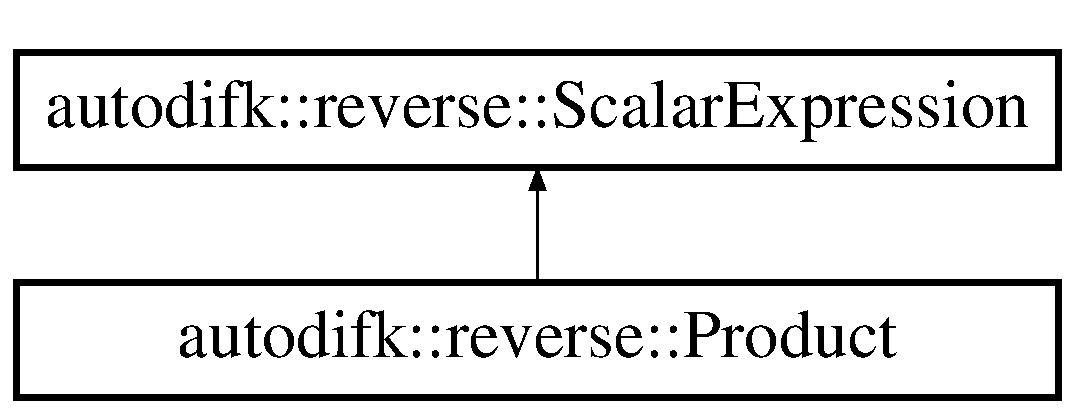
\includegraphics[height=2.000000cm]{classautodifk_1_1reverse_1_1_product}
\end{center}
\end{figure}
\subsection*{Public Types}
\begin{DoxyCompactItemize}
\item 
\hypertarget{classautodifk_1_1reverse_1_1_product_adeb0428c911321657ce9d7f912506f4b}{typedef std\-::shared\-\_\-ptr$<$ \hyperlink{classautodifk_1_1reverse_1_1_product}{Product} $>$ {\bfseries Ptr}}\label{classautodifk_1_1reverse_1_1_product_adeb0428c911321657ce9d7f912506f4b}

\item 
\hypertarget{classautodifk_1_1reverse_1_1_product_a1be85d66996a10650eec57e55e1cfe5f}{typedef std\-::shared\-\_\-ptr$<$ const \\*
\hyperlink{classautodifk_1_1reverse_1_1_product}{Product} $>$ {\bfseries Const\-Ptr}}\label{classautodifk_1_1reverse_1_1_product_a1be85d66996a10650eec57e55e1cfe5f}

\end{DoxyCompactItemize}
\subsection*{Static Public Member Functions}
\begin{DoxyCompactItemize}
\item 
\hypertarget{classautodifk_1_1reverse_1_1_product_ae7353a17d55204b1678385a65d40b8a5}{static Ptr {\bfseries Create} (const std\-::vector$<$ Scalar\-Expression\-::\-Ptr $>$ \&subexpressions)}\label{classautodifk_1_1reverse_1_1_product_ae7353a17d55204b1678385a65d40b8a5}

\item 
\hypertarget{classautodifk_1_1reverse_1_1_product_a0d75bdfb8798feb61644869c1834d782}{static Ptr {\bfseries Create} (const std\-::initializer\-\_\-list$<$ Scalar\-Expression\-::\-Ptr $>$ \&subexpressions)}\label{classautodifk_1_1reverse_1_1_product_a0d75bdfb8798feb61644869c1834d782}

\end{DoxyCompactItemize}
\subsection*{Additional Inherited Members}


\subsection{Detailed Description}


Definition at line 75 of file utils.\-h.



The documentation for this class was generated from the following files\-:\begin{DoxyCompactItemize}
\item 
/home/travis/build/dfridovi/autodifk/include/reverse/utils.\-h\item 
/home/travis/build/dfridovi/autodifk/src/reverse/utils.\-cpp\end{DoxyCompactItemize}

\hypertarget{classautodifk_1_1reverse_1_1_re_l_u}{\section{autodifk\-:\-:reverse\-:\-:Re\-L\-U Class Reference}
\label{classautodifk_1_1reverse_1_1_re_l_u}\index{autodifk\-::reverse\-::\-Re\-L\-U@{autodifk\-::reverse\-::\-Re\-L\-U}}
}
Inheritance diagram for autodifk\-:\-:reverse\-:\-:Re\-L\-U\-:\begin{figure}[H]
\begin{center}
\leavevmode
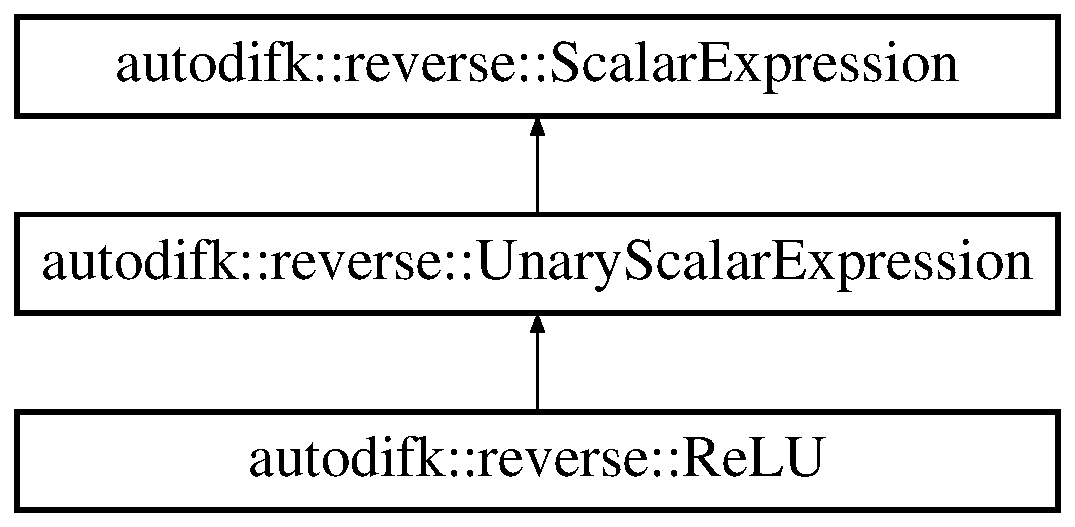
\includegraphics[height=3.000000cm]{classautodifk_1_1reverse_1_1_re_l_u}
\end{center}
\end{figure}
\subsection*{Public Types}
\begin{DoxyCompactItemize}
\item 
\hypertarget{classautodifk_1_1reverse_1_1_re_l_u_a10f0c79f8521e7a77039b6eb6c89411d}{typedef std\-::shared\-\_\-ptr$<$ \hyperlink{classautodifk_1_1reverse_1_1_re_l_u}{Re\-L\-U} $>$ {\bfseries Ptr}}\label{classautodifk_1_1reverse_1_1_re_l_u_a10f0c79f8521e7a77039b6eb6c89411d}

\item 
\hypertarget{classautodifk_1_1reverse_1_1_re_l_u_a58cc1f35f8846f33c62a99e3ada64ab8}{typedef std\-::shared\-\_\-ptr$<$ const \\*
\hyperlink{classautodifk_1_1reverse_1_1_re_l_u}{Re\-L\-U} $>$ {\bfseries Const\-Ptr}}\label{classautodifk_1_1reverse_1_1_re_l_u_a58cc1f35f8846f33c62a99e3ada64ab8}

\end{DoxyCompactItemize}
\subsection*{Static Public Member Functions}
\begin{DoxyCompactItemize}
\item 
\hypertarget{classautodifk_1_1reverse_1_1_re_l_u_ab16e471d11d7d1176661b2304ce5a1fd}{static Ptr {\bfseries Create} (const std\-::vector$<$ Scalar\-Expression\-::\-Ptr $>$ \&subexpressions)}\label{classautodifk_1_1reverse_1_1_re_l_u_ab16e471d11d7d1176661b2304ce5a1fd}

\item 
\hypertarget{classautodifk_1_1reverse_1_1_re_l_u_a7829600acddc4450b67212f94f74f487}{static Ptr {\bfseries Create} (const std\-::initializer\-\_\-list$<$ Scalar\-Expression\-::\-Ptr $>$ \&subexpressions)}\label{classautodifk_1_1reverse_1_1_re_l_u_a7829600acddc4450b67212f94f74f487}

\end{DoxyCompactItemize}
\subsection*{Additional Inherited Members}


\subsection{Detailed Description}


Definition at line 215 of file utils.\-h.



The documentation for this class was generated from the following files\-:\begin{DoxyCompactItemize}
\item 
/home/travis/build/dfridovi/autodifk/include/reverse/utils.\-h\item 
/home/travis/build/dfridovi/autodifk/src/reverse/utils.\-cpp\end{DoxyCompactItemize}

\hypertarget{classautodifk_1_1reverse_1_1_scalar_expression}{\section{autodifk\-:\-:reverse\-:\-:Scalar\-Expression Class Reference}
\label{classautodifk_1_1reverse_1_1_scalar_expression}\index{autodifk\-::reverse\-::\-Scalar\-Expression@{autodifk\-::reverse\-::\-Scalar\-Expression}}
}
Inheritance diagram for autodifk\-:\-:reverse\-:\-:Scalar\-Expression\-:\begin{figure}[H]
\begin{center}
\leavevmode
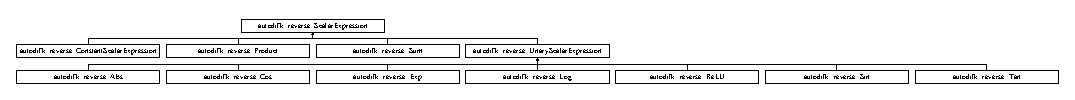
\includegraphics[height=0.895522cm]{classautodifk_1_1reverse_1_1_scalar_expression}
\end{center}
\end{figure}
\subsection*{Public Types}
\begin{DoxyCompactItemize}
\item 
\hypertarget{classautodifk_1_1reverse_1_1_scalar_expression_a99942f407a198eb41cd3229c0a2b8dc3}{typedef std\-::shared\-\_\-ptr\\*
$<$ \hyperlink{classautodifk_1_1reverse_1_1_scalar_expression}{Scalar\-Expression} $>$ {\bfseries Ptr}}\label{classautodifk_1_1reverse_1_1_scalar_expression_a99942f407a198eb41cd3229c0a2b8dc3}

\item 
\hypertarget{classautodifk_1_1reverse_1_1_scalar_expression_a698d78b9940e968e633a026ee1ef14ec}{typedef std\-::shared\-\_\-ptr$<$ const \\*
\hyperlink{classautodifk_1_1reverse_1_1_scalar_expression}{Scalar\-Expression} $>$ {\bfseries Const\-Ptr}}\label{classautodifk_1_1reverse_1_1_scalar_expression_a698d78b9940e968e633a026ee1ef14ec}

\end{DoxyCompactItemize}
\subsection*{Public Member Functions}
\begin{DoxyCompactItemize}
\item 
\hypertarget{classautodifk_1_1reverse_1_1_scalar_expression_a73bd698dda18f14f250b1b6998543c7d}{void {\bfseries Reset} ()}\label{classautodifk_1_1reverse_1_1_scalar_expression_a73bd698dda18f14f250b1b6998543c7d}

\item 
\hypertarget{classautodifk_1_1reverse_1_1_scalar_expression_a2fd311a9ed6d6b577e3d8bfa508f778a}{double {\bfseries Forward\-Pass} ()}\label{classautodifk_1_1reverse_1_1_scalar_expression_a2fd311a9ed6d6b577e3d8bfa508f778a}

\item 
\hypertarget{classautodifk_1_1reverse_1_1_scalar_expression_a77e7fb568d55d68da0338e0d9a10d81f}{void {\bfseries Backward\-Pass} ()}\label{classautodifk_1_1reverse_1_1_scalar_expression_a77e7fb568d55d68da0338e0d9a10d81f}

\end{DoxyCompactItemize}
\subsection*{Public Attributes}
\begin{DoxyCompactItemize}
\item 
\hypertarget{classautodifk_1_1reverse_1_1_scalar_expression_ad164d707dec8ddcda763dd4860260466}{double {\bfseries value}}\label{classautodifk_1_1reverse_1_1_scalar_expression_ad164d707dec8ddcda763dd4860260466}

\item 
\hypertarget{classautodifk_1_1reverse_1_1_scalar_expression_a5abc7368882940867c6bd9dd69d78b0d}{double {\bfseries derivative}}\label{classautodifk_1_1reverse_1_1_scalar_expression_a5abc7368882940867c6bd9dd69d78b0d}

\item 
\hypertarget{classautodifk_1_1reverse_1_1_scalar_expression_a41fd95e27f8091019e6b0f8c0888c283}{const bool {\bfseries is\-\_\-constant}}\label{classautodifk_1_1reverse_1_1_scalar_expression_a41fd95e27f8091019e6b0f8c0888c283}

\end{DoxyCompactItemize}
\subsection*{Protected Member Functions}
\begin{DoxyCompactItemize}
\item 
\hypertarget{classautodifk_1_1reverse_1_1_scalar_expression_ad6e48eecd2f272377d36ff0c96c3d6df}{{\bfseries Scalar\-Expression} (bool is\-\_\-constant=false)}\label{classautodifk_1_1reverse_1_1_scalar_expression_ad6e48eecd2f272377d36ff0c96c3d6df}

\item 
\hypertarget{classautodifk_1_1reverse_1_1_scalar_expression_a6e25133ba71ffb651898c4a1724086fb}{{\bfseries Scalar\-Expression} (double v, bool is\-\_\-constant=false)}\label{classautodifk_1_1reverse_1_1_scalar_expression_a6e25133ba71ffb651898c4a1724086fb}

\item 
\hypertarget{classautodifk_1_1reverse_1_1_scalar_expression_ac4954f13405d688c716d7bb79537e86f}{{\bfseries Scalar\-Expression} (double v, double d)}\label{classautodifk_1_1reverse_1_1_scalar_expression_ac4954f13405d688c716d7bb79537e86f}

\item 
\hypertarget{classautodifk_1_1reverse_1_1_scalar_expression_a80fb01a8e7e88503dd543fc3ac5b3939}{{\bfseries Scalar\-Expression} (const std\-::vector$<$ Scalar\-Expression\-::\-Ptr $>$ \&subexpressions)}\label{classautodifk_1_1reverse_1_1_scalar_expression_a80fb01a8e7e88503dd543fc3ac5b3939}

\item 
\hypertarget{classautodifk_1_1reverse_1_1_scalar_expression_a86a8f5a65b0d6bb0f0ef0a48dab651eb}{{\bfseries Scalar\-Expression} (const std\-::initializer\-\_\-list$<$ Scalar\-Expression\-::\-Ptr $>$ \&subexpressions)}\label{classautodifk_1_1reverse_1_1_scalar_expression_a86a8f5a65b0d6bb0f0ef0a48dab651eb}

\item 
\hypertarget{classautodifk_1_1reverse_1_1_scalar_expression_a7cf1b9db84a62e39294c19fab45958ef}{virtual bool {\bfseries Check\-Subexpressions} () const }\label{classautodifk_1_1reverse_1_1_scalar_expression_a7cf1b9db84a62e39294c19fab45958ef}

\item 
\hypertarget{classautodifk_1_1reverse_1_1_scalar_expression_a358b7c4f8e2425d0e11c0e37c06ff665}{virtual double {\bfseries Forward\-Propagate\-Value} ()=0}\label{classautodifk_1_1reverse_1_1_scalar_expression_a358b7c4f8e2425d0e11c0e37c06ff665}

\item 
\hypertarget{classautodifk_1_1reverse_1_1_scalar_expression_aa25dc105d7ef6eb766383b5b0973957b}{virtual void {\bfseries Backward\-Propagate\-Derivative} ()=0}\label{classautodifk_1_1reverse_1_1_scalar_expression_aa25dc105d7ef6eb766383b5b0973957b}

\end{DoxyCompactItemize}
\subsection*{Protected Attributes}
\begin{DoxyCompactItemize}
\item 
\hypertarget{classautodifk_1_1reverse_1_1_scalar_expression_a948076a05d2f5e36a48ee597c5c91d2d}{std\-::vector\\*
$<$ Scalar\-Expression\-::\-Ptr $>$ {\bfseries subexpressions\-\_\-}}\label{classautodifk_1_1reverse_1_1_scalar_expression_a948076a05d2f5e36a48ee597c5c91d2d}

\end{DoxyCompactItemize}


\subsection{Detailed Description}


Definition at line 55 of file scalar\-\_\-expression.\-h.



The documentation for this class was generated from the following file\-:\begin{DoxyCompactItemize}
\item 
/home/travis/build/dfridovi/autodifk/include/reverse/scalar\-\_\-expression.\-h\end{DoxyCompactItemize}

\hypertarget{classautodifk_1_1reverse_1_1_sin}{\section{autodifk\-:\-:reverse\-:\-:Sin Class Reference}
\label{classautodifk_1_1reverse_1_1_sin}\index{autodifk\-::reverse\-::\-Sin@{autodifk\-::reverse\-::\-Sin}}
}
Inheritance diagram for autodifk\-:\-:reverse\-:\-:Sin\-:\begin{figure}[H]
\begin{center}
\leavevmode
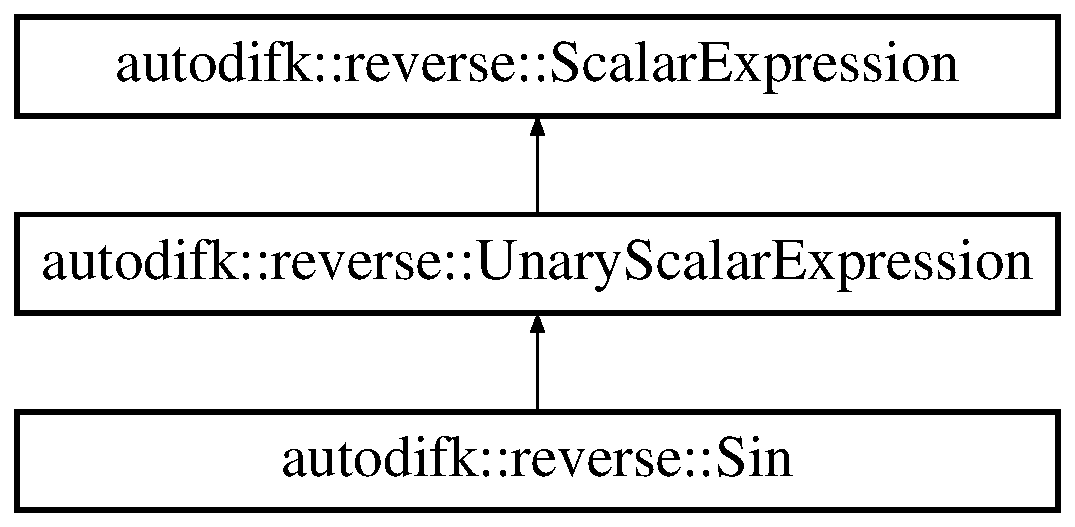
\includegraphics[height=3.000000cm]{classautodifk_1_1reverse_1_1_sin}
\end{center}
\end{figure}
\subsection*{Public Types}
\begin{DoxyCompactItemize}
\item 
\hypertarget{classautodifk_1_1reverse_1_1_sin_a4c07c2b96e3ee3654f7c251e4a08d965}{typedef std\-::shared\-\_\-ptr$<$ \hyperlink{classautodifk_1_1reverse_1_1_sin}{Sin} $>$ {\bfseries Ptr}}\label{classautodifk_1_1reverse_1_1_sin_a4c07c2b96e3ee3654f7c251e4a08d965}

\item 
\hypertarget{classautodifk_1_1reverse_1_1_sin_a2f3caf70999fc6bb5c6c4902e34d018a}{typedef std\-::shared\-\_\-ptr$<$ const \\*
\hyperlink{classautodifk_1_1reverse_1_1_sin}{Sin} $>$ {\bfseries Const\-Ptr}}\label{classautodifk_1_1reverse_1_1_sin_a2f3caf70999fc6bb5c6c4902e34d018a}

\end{DoxyCompactItemize}
\subsection*{Static Public Member Functions}
\begin{DoxyCompactItemize}
\item 
\hypertarget{classautodifk_1_1reverse_1_1_sin_a36c55f4b49a9944af4461c6bebaea991}{static Ptr {\bfseries Create} (const std\-::vector$<$ Scalar\-Expression\-::\-Ptr $>$ \&subexpressions)}\label{classautodifk_1_1reverse_1_1_sin_a36c55f4b49a9944af4461c6bebaea991}

\item 
\hypertarget{classautodifk_1_1reverse_1_1_sin_af3d7caaa42034f30ded25ed7c6f0c0a0}{static Ptr {\bfseries Create} (const std\-::initializer\-\_\-list$<$ Scalar\-Expression\-::\-Ptr $>$ \&subexpressions)}\label{classautodifk_1_1reverse_1_1_sin_af3d7caaa42034f30ded25ed7c6f0c0a0}

\end{DoxyCompactItemize}
\subsection*{Additional Inherited Members}


\subsection{Detailed Description}


Definition at line 95 of file utils.\-h.



The documentation for this class was generated from the following files\-:\begin{DoxyCompactItemize}
\item 
/home/travis/build/dfridovi/autodifk/include/reverse/utils.\-h\item 
/home/travis/build/dfridovi/autodifk/src/reverse/utils.\-cpp\end{DoxyCompactItemize}

\hypertarget{classautodifk_1_1reverse_1_1_sum}{\section{autodifk\-:\-:reverse\-:\-:Sum Class Reference}
\label{classautodifk_1_1reverse_1_1_sum}\index{autodifk\-::reverse\-::\-Sum@{autodifk\-::reverse\-::\-Sum}}
}
Inheritance diagram for autodifk\-:\-:reverse\-:\-:Sum\-:\begin{figure}[H]
\begin{center}
\leavevmode
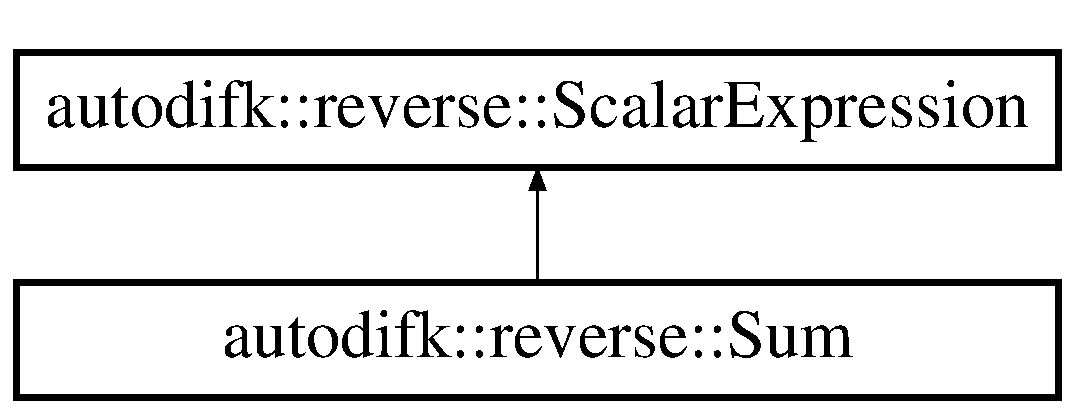
\includegraphics[height=2.000000cm]{classautodifk_1_1reverse_1_1_sum}
\end{center}
\end{figure}
\subsection*{Public Types}
\begin{DoxyCompactItemize}
\item 
\hypertarget{classautodifk_1_1reverse_1_1_sum_ade41b60c006c336813c2df6ffb5d8e70}{typedef std\-::shared\-\_\-ptr$<$ \hyperlink{classautodifk_1_1reverse_1_1_sum}{Sum} $>$ {\bfseries Ptr}}\label{classautodifk_1_1reverse_1_1_sum_ade41b60c006c336813c2df6ffb5d8e70}

\item 
\hypertarget{classautodifk_1_1reverse_1_1_sum_af335e061ffb0ff3bbe20b0889919f448}{typedef std\-::shared\-\_\-ptr$<$ const \\*
\hyperlink{classautodifk_1_1reverse_1_1_sum}{Sum} $>$ {\bfseries Const\-Ptr}}\label{classautodifk_1_1reverse_1_1_sum_af335e061ffb0ff3bbe20b0889919f448}

\end{DoxyCompactItemize}
\subsection*{Static Public Member Functions}
\begin{DoxyCompactItemize}
\item 
\hypertarget{classautodifk_1_1reverse_1_1_sum_a01e19f2d761b38724badc72810914faf}{static Ptr {\bfseries Create} (const std\-::vector$<$ Scalar\-Expression\-::\-Ptr $>$ \&subexpressions)}\label{classautodifk_1_1reverse_1_1_sum_a01e19f2d761b38724badc72810914faf}

\item 
\hypertarget{classautodifk_1_1reverse_1_1_sum_aea5e507fdc009b1e23514a9dc7f753e9}{static Ptr {\bfseries Create} (const std\-::initializer\-\_\-list$<$ Scalar\-Expression\-::\-Ptr $>$ \&subexpressions)}\label{classautodifk_1_1reverse_1_1_sum_aea5e507fdc009b1e23514a9dc7f753e9}

\end{DoxyCompactItemize}
\subsection*{Additional Inherited Members}


\subsection{Detailed Description}


Definition at line 55 of file utils.\-h.



The documentation for this class was generated from the following files\-:\begin{DoxyCompactItemize}
\item 
/home/travis/build/dfridovi/autodifk/include/reverse/utils.\-h\item 
/home/travis/build/dfridovi/autodifk/src/reverse/utils.\-cpp\end{DoxyCompactItemize}

\hypertarget{classautodifk_1_1reverse_1_1_tan}{\section{autodifk\-:\-:reverse\-:\-:Tan Class Reference}
\label{classautodifk_1_1reverse_1_1_tan}\index{autodifk\-::reverse\-::\-Tan@{autodifk\-::reverse\-::\-Tan}}
}
Inheritance diagram for autodifk\-:\-:reverse\-:\-:Tan\-:\begin{figure}[H]
\begin{center}
\leavevmode
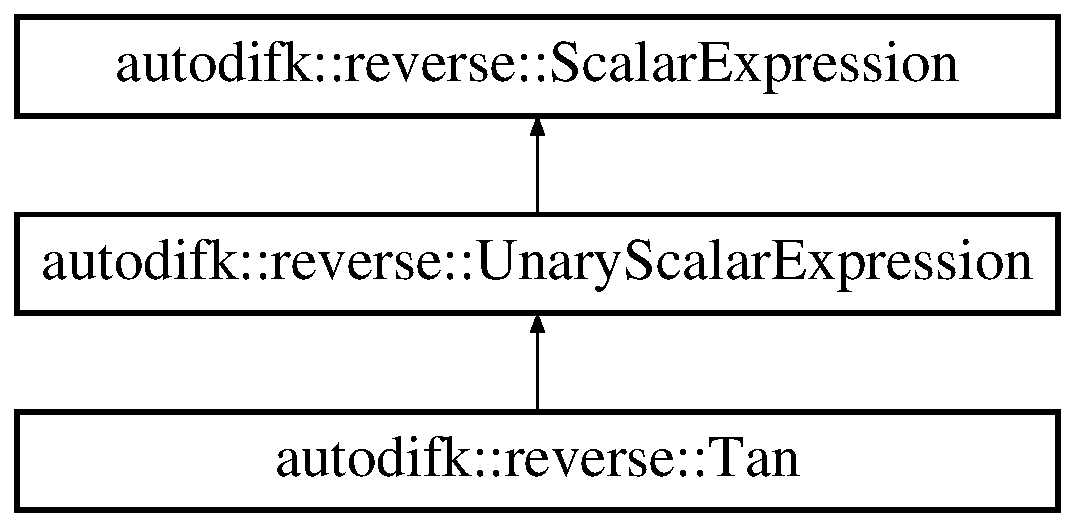
\includegraphics[height=3.000000cm]{classautodifk_1_1reverse_1_1_tan}
\end{center}
\end{figure}
\subsection*{Public Types}
\begin{DoxyCompactItemize}
\item 
\hypertarget{classautodifk_1_1reverse_1_1_tan_aa951354e1c9f764b5e20d3126e174319}{typedef std\-::shared\-\_\-ptr$<$ \hyperlink{classautodifk_1_1reverse_1_1_tan}{Tan} $>$ {\bfseries Ptr}}\label{classautodifk_1_1reverse_1_1_tan_aa951354e1c9f764b5e20d3126e174319}

\item 
\hypertarget{classautodifk_1_1reverse_1_1_tan_aea6f6ac03be50419240104dc4862dc93}{typedef std\-::shared\-\_\-ptr$<$ const \\*
\hyperlink{classautodifk_1_1reverse_1_1_tan}{Tan} $>$ {\bfseries Const\-Ptr}}\label{classautodifk_1_1reverse_1_1_tan_aea6f6ac03be50419240104dc4862dc93}

\end{DoxyCompactItemize}
\subsection*{Static Public Member Functions}
\begin{DoxyCompactItemize}
\item 
\hypertarget{classautodifk_1_1reverse_1_1_tan_a7350ee3a1c6a8990ca3226e7f6404886}{static Ptr {\bfseries Create} (const std\-::vector$<$ Scalar\-Expression\-::\-Ptr $>$ \&subexpressions)}\label{classautodifk_1_1reverse_1_1_tan_a7350ee3a1c6a8990ca3226e7f6404886}

\item 
\hypertarget{classautodifk_1_1reverse_1_1_tan_a602e6795dc44d5b89712b5921acaf618}{static Ptr {\bfseries Create} (const std\-::initializer\-\_\-list$<$ Scalar\-Expression\-::\-Ptr $>$ \&subexpressions)}\label{classautodifk_1_1reverse_1_1_tan_a602e6795dc44d5b89712b5921acaf618}

\end{DoxyCompactItemize}
\subsection*{Additional Inherited Members}


\subsection{Detailed Description}


Definition at line 135 of file utils.\-h.



The documentation for this class was generated from the following files\-:\begin{DoxyCompactItemize}
\item 
/home/travis/build/dfridovi/autodifk/include/reverse/utils.\-h\item 
/home/travis/build/dfridovi/autodifk/src/reverse/utils.\-cpp\end{DoxyCompactItemize}

\hypertarget{classautodifk_1_1reverse_1_1_unary_scalar_expression}{\section{autodifk\-:\-:reverse\-:\-:Unary\-Scalar\-Expression Class Reference}
\label{classautodifk_1_1reverse_1_1_unary_scalar_expression}\index{autodifk\-::reverse\-::\-Unary\-Scalar\-Expression@{autodifk\-::reverse\-::\-Unary\-Scalar\-Expression}}
}
Inheritance diagram for autodifk\-:\-:reverse\-:\-:Unary\-Scalar\-Expression\-:\begin{figure}[H]
\begin{center}
\leavevmode
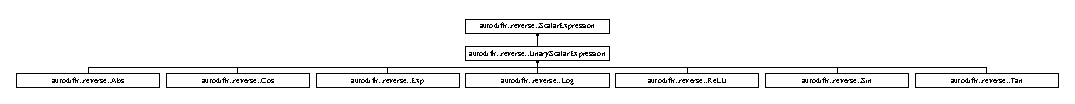
\includegraphics[height=0.948617cm]{classautodifk_1_1reverse_1_1_unary_scalar_expression}
\end{center}
\end{figure}
\subsection*{Protected Member Functions}
\begin{DoxyCompactItemize}
\item 
\hypertarget{classautodifk_1_1reverse_1_1_unary_scalar_expression_a6333034cd7c8e1aa887746161908c390}{virtual bool {\bfseries Check\-Subexpressions} () const }\label{classautodifk_1_1reverse_1_1_unary_scalar_expression_a6333034cd7c8e1aa887746161908c390}

\end{DoxyCompactItemize}
\subsection*{Additional Inherited Members}


\subsection{Detailed Description}


Definition at line 144 of file scalar\-\_\-expression.\-h.



The documentation for this class was generated from the following file\-:\begin{DoxyCompactItemize}
\item 
/home/travis/build/dfridovi/autodifk/include/reverse/scalar\-\_\-expression.\-h\end{DoxyCompactItemize}

%--- End generated contents ---

% Index
\newpage
\phantomsection
\addcontentsline{toc}{chapter}{Index}
\printindex

\end{document}
